\documentclass{article}
\usepackage{amsmath}
\usepackage{graphicx}
\usepackage{float}
\graphicspath{ {.} }

\title{Average Value of a Function}
\author{Alex Katsenelenbogen}

\setlength{\voffset}{-0.75in}

\begin{document}
\begin{center}
      \Large\textbf{Average Value of a Function}\\
      \large\textit{Prepared by Alex Katsenelenbogen}
   \end{center}

\begin{enumerate}


\item 
\vspace{0.4cm}
\begin{equation*}
h(x) = \begin{cases}
$3x+2$ &\text{for $x \leq 2$}\\
$4x$ &\text{for $x2 < x < 5$}\\
$20$ &\text{for $ x \geq 5$}\\
\end{cases}
\end{equation*}

Find the average value of $h(x)$ on the interval $x \epsilon (0,10)$.

\vspace{0.3cm}

\item

\begin{table}[htbp]
\centering
\begin{tabular}[t]{| c | c | c | c | c |}
        \hline
        $x$  & 1 & 4 & 7 & 9 \\
        \hline
        $g(x)$ & 20 & 25 & 35 & 47 \\
        \hline
\end{tabular} 
\end{table}
Given the above values of g(x) at selected points, use the trapezoidal rule to estimate the average value of g(x) on the 
interval, $x \epsilon (1, 9)$.
\vspace{0.3cm} \\

\item 
\begin{equation}
f(x) = \frac{1}{x^2 -1}
\end{equation}
\begin{enumerate}
\item Find the average value, if it exists, of $f(x)$ on the interval (-1, 1).
\item Find the average value, if it exists, of $f(x)$ on the interval (0,2).
\vspace{0.3cm}
\end{enumerate}

\item 
\vspace{0.3cm}
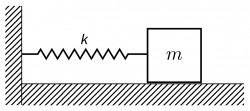
\includegraphics[scale=0.8]{mass-spring}
\vspace{0.3cm} \\
A $5$ kg mass is in an equilibrium position at $x=0$. The mass is pulled outward to the right, and released at time $t=0$, where t is measured in seconds. It begins to move in a sinusoidal motion about the equilibrium position; the motion can be modeled by the equation $x(t)=2cos(\omega t)$ where the frequency $\omega$ is equal to $\sqrt{\frac{k}{m}}$, the spring constant $k$ is 125 N/m, and $x$ represents the horizontal distance from equilibrium.

\textbf{Note}: a positive $x$ value means that the mass is to the right of equilibrium, and a negative $x$ value means that the mass is to the left of equilibrium.

\begin{enumerate}
\item What is the average value of the mass's x-position for the first $\frac{2\pi}{5}$ seconds of motion?
\item What is the average value of the mass's absolute distance from equilibrium for the
first $\frac{2\pi}{5}$  seconds of motion?
\item What is the average value of the mass's velocity for
the first $\frac{2\pi}{5}$ seconds of motion?
\end{enumerate}
\end{enumerate}
\end{document}
